\documentclass[10pt,aspectratio=169]{beamer}

%====================
% Packages
%====================
\usepackage[utf8]{inputenc}
\usepackage[T1]{fontenc}
\usepackage[provide=*,french]{babel}
\usepackage{lmodern}
\usepackage{amsmath,amssymb}
\usepackage{booktabs}
\usepackage{array}
\usepackage{colortbl}
\usepackage{pifont}
\usepackage{tikz}
\usetikzlibrary{positioning,arrows.meta,shapes.geometric,calc}

%====================
% Style
%====================
\usetheme{Madrid}
\usecolortheme{default}
\setbeamertemplate{navigation symbols}{}
\setbeamertemplate{blocks}[rounded][shadow=true]

\definecolor{DeepBlue}{RGB}{18,45,83}
\definecolor{AccentBlue}{RGB}{30,90,160}
\definecolor{SoftBlue}{RGB}{225,238,250}
\definecolor{Gold}{RGB}{236,178,46}
\definecolor{DarkGray}{RGB}{58,65,76}
\definecolor{LightGray}{RGB}{245,247,250}
\definecolor{SuccessGreen}{RGB}{49,132,91}
\definecolor{FutureGray}{RGB}{150,158,170}

\setbeamercolor{palette primary}{bg=DeepBlue,fg=white}
\setbeamercolor{palette secondary}{bg=AccentBlue,fg=white}
\setbeamercolor{palette tertiary}{bg=DeepBlue,fg=white}
\setbeamercolor{frametitle}{bg=DeepBlue,fg=white}
\setbeamercolor{title}{fg=white}
\setbeamercolor{subtitle}{fg=SoftBlue}
\setbeamercolor{block title}{bg=AccentBlue,fg=white}
\setbeamercolor{block body}{bg=SoftBlue,fg=black}
\setbeamercolor{normal text}{fg=DarkGray}

\setbeamertemplate{footline}{%
  \leavevmode%
  \hbox{%
  \begin{beamercolorbox}[wd=.78\paperwidth,ht=2.5ex,dp=1ex,leftskip=2ex]{palette primary}%
    \insertshorttitle
  \end{beamercolorbox}%
  \begin{beamercolorbox}[wd=.22\paperwidth,ht=2.5ex,dp=1ex,center]{palette secondary}%
    \insertframenumber/\inserttotalframenumber
  \end{beamercolorbox}}%
}

\newcommand{\keyword}[1]{\textcolor{AccentBlue}{\textbf{#1}}}
\newcommand{\week}[1]{\textcolor{Gold}{\textbf{#1}}}
\newcommand{\done}{\textcolor{SuccessGreen}{\ding{51}}}
\newcommand{\current}{\textcolor{Gold}{\raisebox{-0.15ex}{\Large\ding{43}}}}

\tikzset{
  flowbox/.style={
    draw=AccentBlue,
    fill=SoftBlue,
    rounded corners=2pt,
    minimum height=1.15cm,
    text width=2.6cm,
    align=center,
    font=\small
  },
  currentbox/.style={
    draw=Gold,
    very thick,
    fill=yellow!12,
    rounded corners=2pt,
    minimum height=1.15cm,
    text width=2.6cm,
    align=center,
    font=\small
  },
  arrow/.style={-{Latex[length=2.2mm]},thick,draw=DarkGray}
}

%====================
% Informations
%====================
\title[Consolidation de l'IM et Cover-2]{Consolidation de la marge initiale\\et extension de la cascade de défaut}
\subtitle{}
\author{}
\institute{\Large\textbf{Quant Factory}}
\date{Juin 2026}

\begin{document}

%====================
\begin{frame}
  \titlepage
\end{frame}

%====================
\begin{frame}{Contexte du projet}
  \begin{columns}[T,onlytextwidth]
    \column{0.48\textwidth}
    \begin{block}{Point de départ}
      Un moteur de \keyword{marge initiale} existe pour le marché obligataire
      souverain marocain :
      \begin{itemize}
        \item scénarios historiques filtrés par EWMA ;
        \item Expected Shortfall à 99\,\% ;
        \item horizon de liquidation de 5 jours ;
        \item composantes courante et stress.
      \end{itemize}
    \end{block}

    \column{0.48\textwidth}
    \begin{block}{Objectif du stage}
      Consolider la première ligne de défense, puis prolonger le moteur :
      \begin{enumerate}
        \item validation indépendante de l'IM ;
        \item fonds de défaut mutualisé \keyword{Cover-2} ;
        \item add-ons de liquidité et de décorrélation.
      \end{enumerate}
    \end{block}
  \end{columns}

  \vspace{0.35cm}
  \centering
  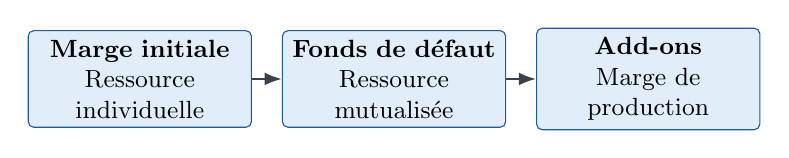
\begin{tikzpicture}[node distance=0.38cm]
    \node[flowbox] (im) {\textbf{Marge initiale}\\Ressource individuelle};
    \node[flowbox,right=of im] (df) {\textbf{Fonds de défaut}\\Ressource mutualisée};
    \node[flowbox,right=of df] (addons) {\textbf{Add-ons}\\Marge de production};
    \draw[arrow] (im) -- (df);
    \draw[arrow] (df) -- (addons);
  \end{tikzpicture}
\end{frame}

%====================
\begin{frame}{Démarche de consolidation de la marge initiale}
  \centering
  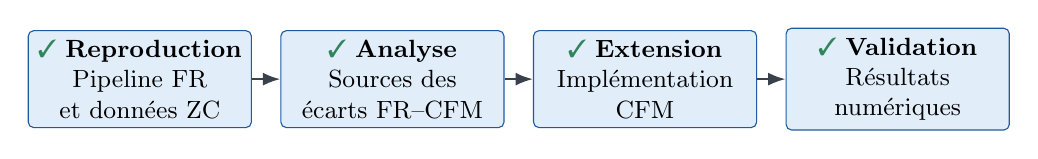
\begin{tikzpicture}[node distance=0.36cm]
    \node[flowbox] (a) {\done\ \textbf{Reproduction}\\Pipeline FR et données ZC};
    \node[flowbox,right=of a] (b) {\done\ \textbf{Analyse}\\Sources des écarts FR--CFM};
    \node[flowbox,right=of b] (c) {\done\ \textbf{Extension}\\Implémentation CFM};
    \node[flowbox,right=of c] (d) {\done\ \textbf{Validation}\\Résultats numériques};
    \draw[arrow] (a) -- (b);
    \draw[arrow] (b) -- (c);
    \draw[arrow] (c) -- (d);
  \end{tikzpicture}

  \vspace{0.55cm}
  \begin{columns}[T,onlytextwidth]
    \column{0.48\textwidth}
    \begin{block}{Approche Full Revaluation}
      Chaque scénario choque les piliers de la courbe ZC. La courbe stressée
      est interpolée, puis chaque obligation est entièrement revalorisée.
    \end{block}

    \column{0.48\textwidth}
    \begin{block}{Approche Cash-Flow Mapping}
      Chaque cash-flow est décomposé sur ses deux piliers voisins avec des
      poids préservant sa valeur et sa variance historique.
    \end{block}
  \end{columns}

  \vspace{0.2cm}
  \centering
  \keyword{Résultat :} une seconde implémentation indépendante confirme
  l'analyse théorique des écarts.
\end{frame}

%====================
\begin{frame}{FR et CFM : même risque, propagation différente}
  \renewcommand{\arraystretch}{1.35}
  \centering
  \begin{tabular}{>{\bfseries}p{2.7cm}p{4.5cm}p{4.5cm}}
    \toprule
    & Full Revaluation (FR) & Cash-Flow Mapping (CFM) \\
    \midrule
    Entrées
      & Courbe ZC courante et returns par pilier
      & Mêmes courbes, returns et scénarios \\
    Propagation
      & Interpolation de la courbe stressée
      & Mapping des cash-flows sur les piliers \\
    Pondération
      & Facteurs d'actualisation
      & Variance--corrélation historique \\
    PnL
      & Revalorisation complète des instruments
      & Agrégation des expositions mappées \\
    \bottomrule
  \end{tabular}

  \vspace{0.45cm}
  \begin{block}{Lecture}
    Les deux méthodes coïncident sous un choc parallèle. Les écarts
    apparaissent avec les mouvements de \keyword{pente}, de
    \keyword{courbure} ou de \keyword{twist}.
  \end{block}
\end{frame}

%====================
\begin{frame}{Validation analytique de l'implémentation CFM}
  Pour un cash-flow situé entre les piliers $T_n$ et $T_{n+1}$ :

  \[
    \Delta \mathrm{PnL}^{(s)}
    =
    \mathrm{MVCF}
    \left(w_n^{FR}-w_n^{CFM}\right)
    \left(R^{(s)}(T_n)-R^{(s)}(T_{n+1})\right).
  \]

  \begin{columns}[T,onlytextwidth]
    \column{0.49\textwidth}
    \begin{block}{Test réalisé}
      \begin{itemize}
        \item calcul direct : $\mathrm{PnL}_{FR}-\mathrm{PnL}_{CFM}$ ;
        \item calcul par la formule analytique ;
        \item comparaison scénario par scénario.
      \end{itemize}
    \end{block}

    \column{0.47\textwidth}
    \begin{block}{Diagnostic numérique}
      \[
        \Delta \mathrm{PnL}_{direct}=-3{,}383725
      \]
      \[
        \Delta \mathrm{PnL}_{formule}=-3{,}383725
      \]
      \[
        \left|\Delta_{\mathrm{num}}\right|\approx 4{,}4\times10^{-14}
      \]
    \end{block}
  \end{columns}

  \centering
  \done\quad \textbf{La relation théorique est confirmée à la précision machine.}
\end{frame}

%====================
\begin{frame}{Passage à la seconde ligne : fonds de défaut Cover-2}
  \begin{columns}[T,onlytextwidth]
    \column{0.50\textwidth}
    \begin{block}{Pourquoi un fonds de défaut ?}
      La marge initiale couvre les pertes dans des conditions normales
      sévères. Sous un stress extrême, une perte résiduelle peut subsister
      après consommation de l'IM.
    \end{block}

    \column{0.46\textwidth}
    \begin{block}{Principe Cover-2}
      Dimensionner une ressource mutualisée capable de couvrir,
      dans un même scénario, les deux plus grandes pertes résiduelles
      parmi les membres compensateurs.
    \end{block}
  \end{columns}

  \vspace{0.45cm}
  \centering
  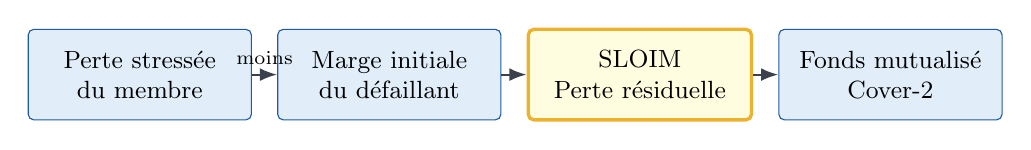
\begin{tikzpicture}[node distance=0.32cm]
    \node[flowbox] (loss) {Perte stressée\\du membre};
    \node[flowbox,right=of loss] (margin) {Marge initiale\\du défaillant};
    \node[currentbox,right=of margin] (sloim) {SLOIM\\Perte résiduelle};
    \node[flowbox,right=of sloim] (cover) {Fonds mutualisé\\Cover-2};
    \draw[arrow] (loss) -- node[above,font=\scriptsize]{moins} (margin);
    \draw[arrow] (margin) -- (sloim);
    \draw[arrow] (sloim) -- (cover);
  \end{tikzpicture}
\end{frame}

%====================
\begin{frame}{Calcul Cover-2 implémenté}
  Pour chaque membre $i$ et chaque scénario de stress $s$ :

  \[
    L_i(s)=\max\!\left(-\mathrm{PnL}_i(s),0\right),
    \qquad
    \mathrm{SLOIM}_i(s)=\max\!\left(L_i(s)-IM_i,0\right).
  \]

  \[
    \mathrm{Cover2}(s)
      =\mathrm{SLOIM}_{(1)}(s)+\mathrm{SLOIM}_{(2)}(s),
    \qquad
    DF=\max_s \mathrm{Cover2}(s).
  \]

  \vspace{0.25cm}
  \centering
  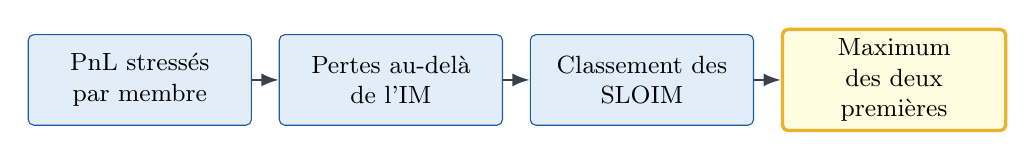
\begin{tikzpicture}[node distance=0.34cm]
    \node[flowbox] (pnl) {PnL stressés\\par membre};
    \node[flowbox,right=of pnl] (res) {Pertes au-delà\\de l'IM};
    \node[flowbox,right=of res] (rank) {Classement des\\SLOIM};
    \node[currentbox,right=of rank] (max) {Maximum\\des deux premières};
    \draw[arrow] (pnl) -- (res);
    \draw[arrow] (res) -- (rank);
    \draw[arrow] (rank) -- (max);
  \end{tikzpicture}

  \vspace{0.35cm}
  \keyword{Travail effectué :} portefeuilles multi-membres, scénario
  contraignant, contrôles de cohérence et dimensionnement du fonds.
\end{frame}

%====================
\begin{frame}{Allocation des contributions entre les membres}
  \begin{columns}[T,onlytextwidth]
    \column{0.48\textwidth}
    \begin{block}{Principe réglementaire}
      La CCP fixe une contribution minimale et répartit le fonds
      proportionnellement à l'exposition de chaque membre.
    \end{block}

    \column{0.48\textwidth}
    \begin{block}{Prototype étudié}
      Comparaison de deux clés d'allocation :
      \begin{itemize}
        \item poids fondés sur la marge initiale ;
        \item poids fondés sur la SLOIM.
      \end{itemize}
    \end{block}
  \end{columns}

  \[
    DF^{buffer}=DF(1+b),
    \qquad
    C_i=C_i^{min}
      +w_i\left(DF^{buffer}-\sum_j C_j^{min}\right).
  \]

  \begin{alertblock}{Point méthodologique à finaliser}
    Le buffer de 10\,\% et le plancher de 2\,\% utilisés dans le prototype
    sont des hypothèses de travail. Leur calibration doit être documentée
    et testée en sensibilité.
  \end{alertblock}
\end{frame}

%====================
\begin{frame}{Tableau de suivi du stage}
  \small
  \renewcommand{\arraystretch}{1.45}
  \centering
  \begin{tabular}{p{1.25cm}p{7.5cm}p{2.5cm}}
    \toprule
    \textbf{Période} & \textbf{Objectif} & \textbf{Statut} \\
    \midrule
    S1--S2
      & Prise en main, reproduction de l'IM et validation CFM
      & \done\ Terminé \\
    \rowcolor{yellow!12}
    S3--S5
      & Fonds de défaut : SLOIM, Cover-2 et allocation des contributions
      & \current\ \textbf{Je suis ici} \\
    S6--S7
      & Marge de production : add-ons de liquidité et de décorrélation
      & \textcolor{FutureGray}{À venir} \\
    S8
      & Consolidation et documentation
      & \textcolor{FutureGray}{À venir} \\
    \bottomrule
  \end{tabular}

  \vspace{0.45cm}
  \begin{block}{Position actuelle}
    Le dimensionnement Cover-2 est opérationnel. Le travail immédiat porte
    sur la \keyword{clé d'allocation}, sa calibration et les tests de
    sensibilité avant la rédaction de la note méthodologique.
  \end{block}
\end{frame}

%====================
\begin{frame}{Planning synthétique}
  \centering
  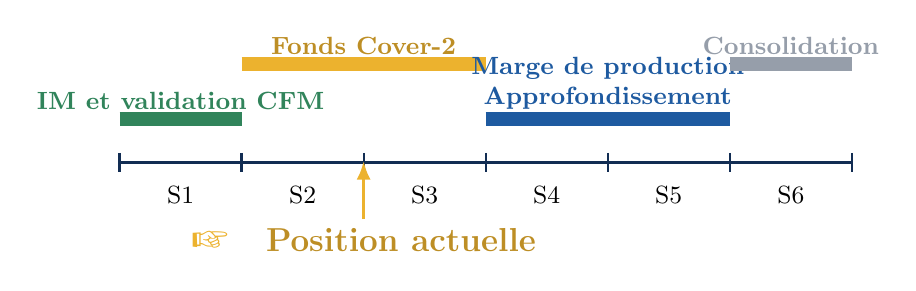
\begin{tikzpicture}[x=1.55cm,y=1cm]
    \draw[very thick,DeepBlue] (0,0) -- (6,0);
    \foreach \x in {0,1,2,3,4,5,6}{
      \draw[DeepBlue,thick] (\x,0.12) -- (\x,-0.12);
    }
    \foreach \x/\lab in {0.5/S1,1.5/S2,2.5/S3,3.5/S4,4.5/S5,5.5/S6}{
      \node[below=0.18cm,font=\small] at (\x,0) {\lab};
    }

    \draw[line width=5pt,SuccessGreen] (0,0.55) -- (1,0.55);
    \node[above,font=\small\bfseries,text=SuccessGreen,align=center] at (0.5,0.55)
      {IM et validation CFM};

    \draw[line width=5pt,Gold] (1,1.25) -- (3,1.25);
    \node[above,font=\small\bfseries,text=Gold!80!black] at (2,1.25)
      {Fonds Cover-2};

    \draw[line width=5pt,AccentBlue] (3,0.55) -- (5,0.55);
    \node[above,font=\small\bfseries,text=AccentBlue,align=center] at (4,0.55)
      {Marge de production\\Approfondissement};

    \draw[line width=5pt,FutureGray] (5,1.25) -- (6,1.25);
    \node[above,font=\small\bfseries,text=FutureGray] at (5.5,1.25)
      {Consolidation};

    \node[text=Gold!80!black,font=\large\bfseries,align=center] at (2,-1.0)
      {\current\quad Position actuelle};
    \draw[-{Latex[length=2.4mm]},very thick,Gold] (2,-0.72) -- (2,0.02);
  \end{tikzpicture}

  \vspace{0.3cm}
  \begin{block}{Prochaine transition}
    Une fois le fonds stabilisé et documenté, le moteur sera prolongé vers
    la marge de production complète : IM de base + add-ons.
  \end{block}
\end{frame}

%====================
\begin{frame}{Suite du stage : marge de production}
  \begin{columns}[T,onlytextwidth]
    \column{0.48\textwidth}
    \begin{block}{Add-on de liquidité}
      Couvrir le coût supplémentaire lié à la liquidation de positions
      concentrées ou peu liquides sur le marché obligataire marocain.
    \end{block}

    \column{0.48\textwidth}
    \begin{block}{Add-on de décorrélation}
      Couvrir le risque que les relations historiques entre facteurs de
      risque se dégradent en période de stress.
    \end{block}
  \end{columns}

  \vspace{0.5cm}
  \[
    IM_{\text{production}}
      =
    IM_{\text{base}}
      + AddOn_{\text{liquidité}}
      + AddOn_{\text{décorrélation}},
  \]
  sous réserve d'une règle d'agrégation évitant le double comptage.
\end{frame}

%====================
\begin{frame}{Références méthodologiques}
  \begin{itemize}
    \item \textbf{EMIR, article 42} : fonds de défaut préfinancé et
      contributions proportionnelles aux expositions des membres.
    \item \textbf{Règlement délégué (UE) nº 153/2013, article 53} :
      scénarios de stress et couverture des deux plus grandes expositions.
    \item \textbf{CPMI--IOSCO, PFMI, principe 4} :
      cadre international du risque de crédit et du standard Cover-2.
    \item \textbf{Eurex Clearing, méthodologie du Default Fund} :
      exemple opérationnel d'allocation fondée sur la perte stressée.
    \item \textbf{Note Fonds de défaut -- Quant Factory} :
      méthodologie de référence utilisée pour le prototype.
  \end{itemize}

\end{frame}

\end{document}
